\begin{frame}[fragile,shrink=30]
   \frametitle{Choropleth}
   \begin{lstlisting}[language=Python]
    v = Visualizer('path/to/file.csv')
    fig = v.choropleth(title = '...',
                  features = 'all',
                  countries = 'all')
    fig.show() # for inline display (in browsers for example)
    \end{lstlisting}
    \begin{center}
        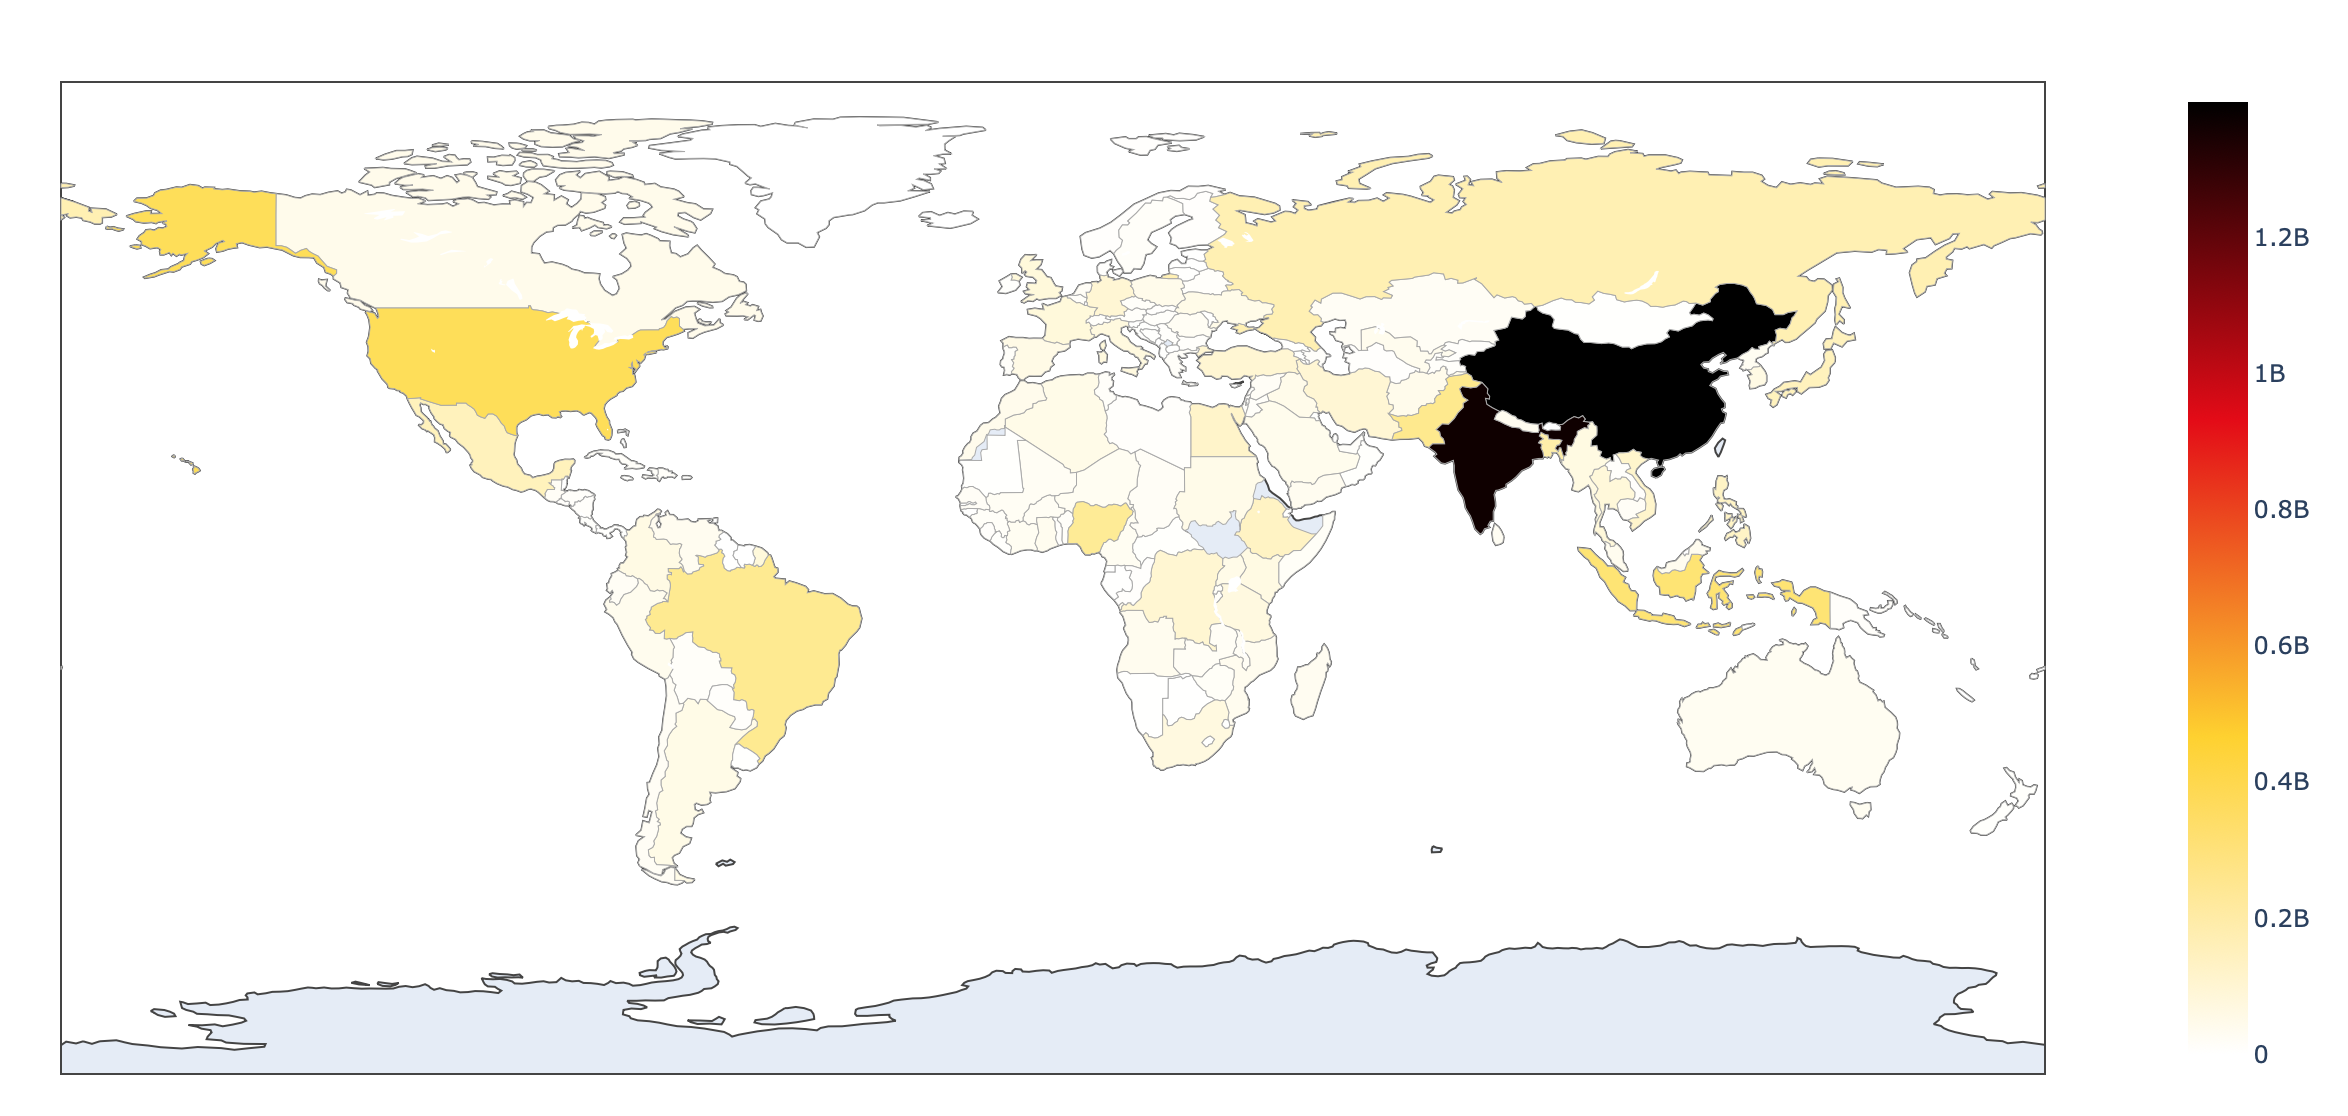
\includegraphics[scale=0.4]{beamer/inc/graphics/choropleth.png} 
    \end{center}
\end{frame}

\begin{frame}[fragile,shrink=30]
  \frametitle{Heatmap}
  \begin{lstlisting}[language=Python]
  v = Visualizer('path/to/file.csv')
  fig = v.heatmap(countries='all', features='all',
                    method='pearson', mask=True,
                    title='', xlabel='', ylabel='')
  fig.show() #for inline display (in browsers for example)
  \end{lstlisting}
  \begin{center}
    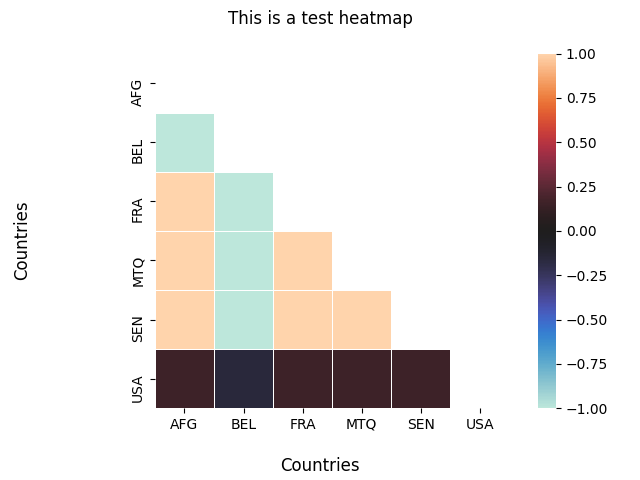
\includegraphics[scale=0.6]{beamer/inc/graphics/heatmap.png}
    \end{center}
\end{frame}

\begin{frame}[fragile,shrink=30]
  \frametitle{Time Series Plot}
  \begin{lstlisting}[language=Python]
    v = Visualizer('path/to/file.csv')
    fig = v.line(countries='all', features='all',
              title='', xlabel='', ylabel='', 
              legend=False)
    fig.show() # for inline display (in browsers for example)
      \end{lstlisting}
    \begin{center}
    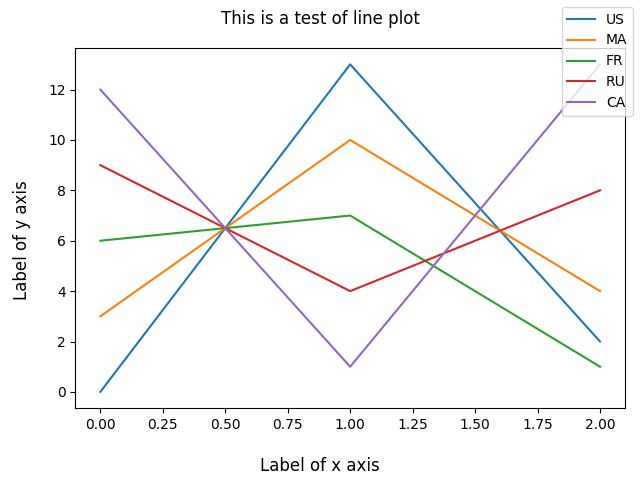
\includegraphics[scale=0.6]{beamer/inc/graphics/line.png}
    \end{center}
\end{frame}

\begin{frame}[fragile,shrink=30]
  \frametitle{Histogram}
    \begin{lstlisting}[language=Python]
    v = Visualizer('path/to/file.csv')
    fig = v.histogram(countries='all', features='all',
                    title='', xlabel='', ylabel='', 
                    legend=False)
    fig.show() # for inline display (in browsers for example)
    \end{lstlisting}
    \begin{center}
    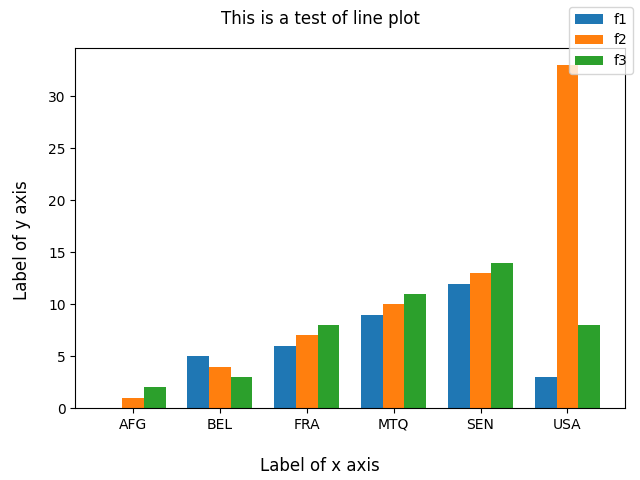
\includegraphics[scale=0.6]{beamer/inc/graphics/histogram.png}
    \end{center}
\end{frame}

